\documentclass[14pt, a4paper]{article}

%Пакеты для русского  языка
\usepackage[T1,T2A]{fontenc}
\usepackage[utf8]{inputenc}
\usepackage[russian]{babel}

%Пакет расширенной математики
\usepackage{amsmath}
\usepackage{amsfonts}

%Графический пакет
\usepackage{pgfplots}
\usepackage{circuitikz}
\ctikzset{resistor = european}
\usetikzlibrary{arrows}

\pgfplotsset{compat = newest, width=77mm}
\usetikzlibrary{positioning, arrows.meta}
\usepgfplotslibrary{fillbetween}
\usepackage{subfig}

%Пакеты для отступов
\usepackage{geometry}
\geometry{top=20mm, right=15mm, bottom=20mm, left=15mm}
\usepackage{indentfirst}

%Пакет для расширенных таблиц
\usepackage{array}
\usepackage{multirow}

%Гиперссылки
\usepackage{hyperref}
\definecolor{linkcolor}{HTML}{799B03} % цвет ссылок
\definecolor{urlcolor}{HTML}{799B03} % цвет гиперссылок
\hypersetup{pdfstartview=FitH,  linkcolor=linkcolor,urlcolor=urlcolor, colorlinks=true}

%Всевозможные картинки
\usepackage{wrapfig}
\usepackage{graphicx}
\usepackage{mathtext}
\usepackage{amsmath}
\usepackage{siunitx}
\usepackage{rotating}
\usepackage{graphicx,xcolor}

\graphicspath{{pictures/}}
\usepackage{wrapfig}
\usepackage{graphicx}
\usepackage{mathtext}
\usepackage{amsmath}
\usepackage{siunitx} % Required for alignment
\usepackage{multirow}
\usepackage{rotating}
\usepackage{afterpage}
\usepackage[T1,T2A]{fontenc}
\usepackage[russian]{babel}
\usepackage{caption}
\usepackage[arrowdel]{physics}
\usepackage{booktabs}
\usepackage{lscape}

\begin{document}

\begin{titlepage}
    \begin{center}
    
    \Large МОСКОВСКИЙ ФИЗИКО-ТЕХНИЧЕСКИЙ ИНСТИТУТ \\ (НАЦИОНАЛЬНЫЙ ИССЛЕДОВАТЕЛЬСКИЙ УНИВЕРСИТЕТ)
    \vspace{0.3cm}
    
    \Large Физтех-школа радиотехники и компьютерных технологий
    \vspace{1cm}

  \begin{figure}[h]
    \centering
    
\includegraphics[width=0.5\linewidth]{logo.png}
    \label{fig:mpr} 
  \end{figure}

    \Huge {\bfseries Лабораторная работа № 4.5.3} 
    
СКАНИРУЮЩИЙ ИНТЕРФЕРОМЕТР

    \vspace{1cm}
    
    \begin{flushright}
{\LARGE Авторы:\\ Голенских Никита \\ Аль Мажариш Гасем \\ гр. Б01-205}
\end{flushright}
    
    \vspace{\fill}
    \Large Долгопрудный 2024
    
    \end{center}
    \end{titlepage}

   
    
    \tableofcontents
    \newpage
    
\section{Аннотация}

\subsection{Цель работы} 
Знакомство с устройством и работой газового лазера непрерывного действия, со спектральными характеристиками лазерного излучения, а также с устройством и принципом действия сканирующего интерферометра Фабри—Перо.

\subsection{Оборудование}
He-Ne лазер с блоком питания; сканирующий интерферометр Фабри-Перо; поляроид; пластинка $\lambda/4$; линза; фотодиод; электронный осциллограф.


\section{Теоретическая часть}
\subsection{Спектр лазера}
В He–Ne-лазерах используются резонаторы, фактически представляющие собой интерферометр Фабри—Перо. Излучение распространяется вдоль оси интерферометра. При этом генерируются моды (типы колебаний), для которых на длине резонатора укладывается целое число полуволн
($L$ -- база интерферометра):

\begin{equation}
    2L=m\lambda
    \label{eq:mode_distance_lambda}
\end{equation}

Из этой формулы получаем разность частот соседних мод

\begin{equation}
    \nu_{m+1} - \nu_{m} = \frac{c}{2L}
    \label{eq:mode_distance_freq}
\end{equation}

Для интерферометра с базой L = 0,6 м межмодовое расстояние равно 250 МГц. В то же время спектральная линия рабочего перехода неона имеет ширину порядка 1500 МГц, поэтому возможна одновременная генерация нескольких мод. Рис. \ref{fig:multimodes} иллюстрирует увеличение числа мод генерации лазера с ростом усиления активной среды.

\begin{figure}[h]
    \center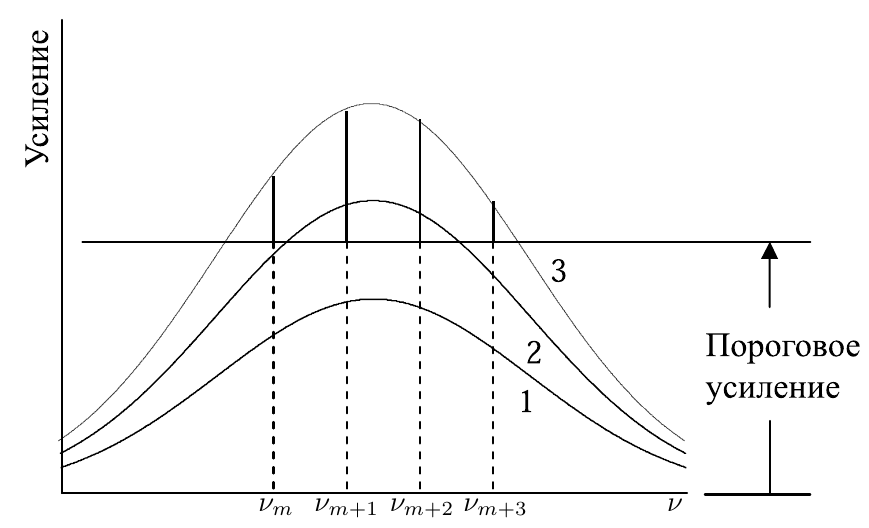
\includegraphics[width = 0.6\linewidth]{multimodes.png}
    \caption{Увеличение числа генерирующих мод при увеличении усиления}\label{fig:multimodes}
\end{figure}

При небольшом усилении (кривая 1) генерации нет. В случае 2 генерация происходит только на 2 частотах $\nu_{m+1}$ и $\nu_{m+2}$ , расположенных вблизи центра спектральной линии. Если усиление определяется кривой 3, генерация возникает на четырёх частотах от $\nu_m$ до $\nu_{m+3}$. Говорят, что в этом случае лазер одновременно работает на четырёх модах.

Для гелий-неонового лазера с достаточно длинной трубкой на переходе 632.8 нм многомодовая генерация является обычным режимом работы.

\subsection{Сканирующий интерферометр}
Для исследования межмодового состава излучения He–Ne-лазера в работе используется сканирующий интерферометр, представляющий собой высокодобротный интерферометр Фабри–Перо с периодически изменяемой базой. Его устройство схематически показано на рис.  \ref{fig:interferometr}.

\newpage

\begin{figure}[h]
    \center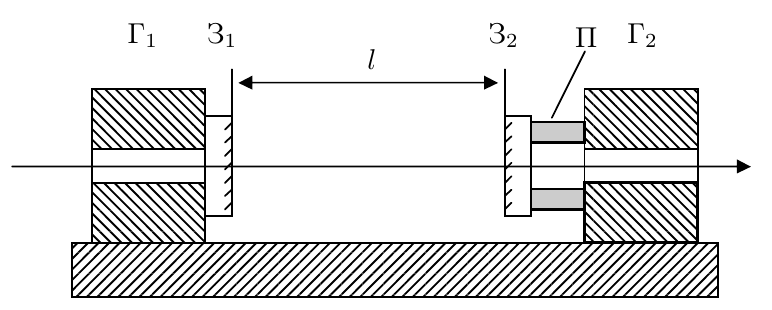
\includegraphics[width = 0.6\linewidth]{interferometr.png}
    \caption{Устройство сканирующего интерферометра}\label{fig:interferometr}
\end{figure}

Если вдоль оси интерферометра распространяется световое излучение с длиной волны $\lambda$, то при выполнении условия

\begin{equation}
    2l=m\lambda
    \label{eq:fabri_resonanse}
\end{equation}
возникает резонанс, и внешнее излучение полностью проходит через интерферометр. Собственные моды интерферометра отличаются по частоте на величину

\begin{equation}
    \Delta \nu = \frac{c}{2l}
    \label{eq:mode_distance_freq_fabri}
\end{equation}
или в единицах $\lambda$
\begin{equation}
    \Delta \lambda_{\text{си}} = \frac{\lambda}{m} = \frac{\lambda^2}{2l}
    \label{eq:mode_distance_lambda_fabri}
\end{equation}

Пьезокерамический элемент П периодически изменяет длину интерферометра на величину порядка $\lambda$, благодаря чему ``плавает'' $l$, и, соответственно, частота сканирования интерферометра. Если амплитуда колебания зеркала небольшая ($\leq \lambda/2$), то размытые спектральные пики не перекрываются, и мы получаем одинарную развертку. При больших амплитудах развертка клонируется (начинается сканирование следующей модой интерферометра), и получается многократная развертка спектра (см. рис. \ref{fig:clone_spectrum})

\begin{figure}[h]
    \center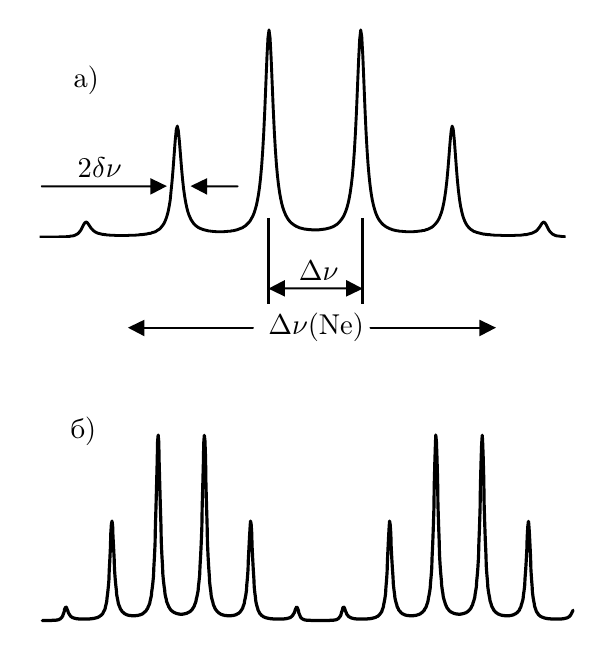
\includegraphics[width = 0.6\linewidth]{clone_spectrum.png}
    \caption{Раздвоение развертки при большой амплитуде колебания зеркала}\label{fig:clone_spectrum}
\end{figure}

\newpage
\subsection{Экспериментальная установка}
\begin{figure}[h]
    \center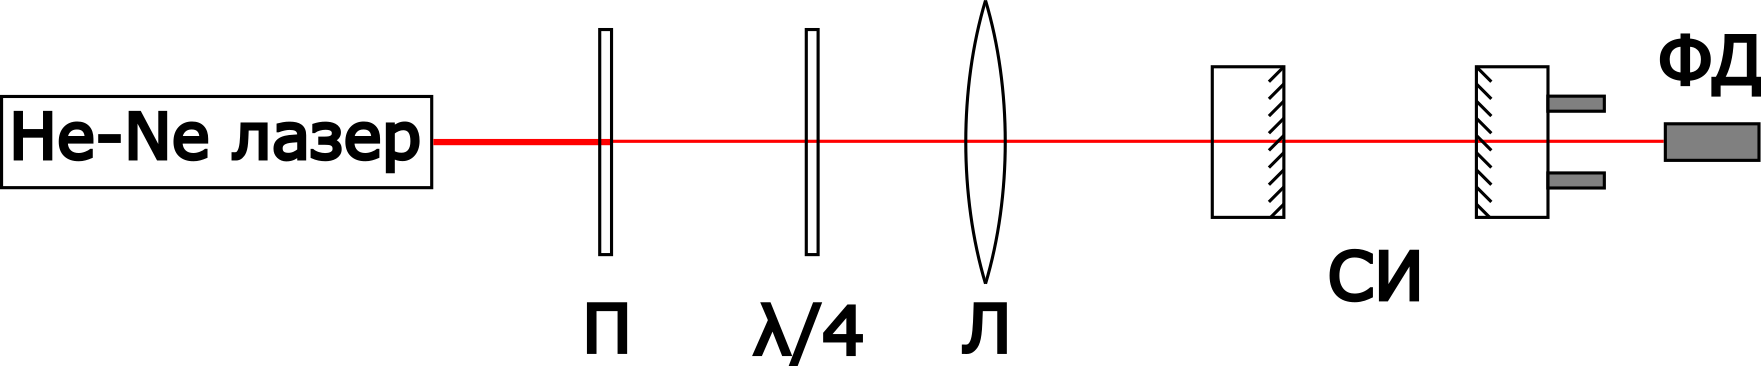
\includegraphics[width=0.9\linewidth]{ustanovka.png}
    \caption{Схема установки}\label{fig:ustanovka}
\end{figure}

Луч лазера проходит через поляризационную развязку, состоящую из поляроида и пластинки $\lambda/4$. Главное направление пластинки $\lambda/4$ повернуто на $45^\circ$ относительно главного направления поляроида, вследствии чего луч на выходе приобретает циркулярную поляризацию. При отражении от линзы или зеркал, круговая поляризация меняет направление, и после прохождения через пластинку $\lambda/4$ приобретает линейную поляризацию, перпендикулярную разрешенному направлению поляроида. Таким путем ограничивается световой поток обратно в лазер, благодаря чему добивается лучшее усиление в трубке лазера.

Линза уменьшает расхождения пучка, поступающего на вход интерферометра. Амплитуда колебания заднего зеркала регулируется через блок питания, а сигнал с фотодиода разворачивается на осциллографе, давая спектр излучения.
 
\section{Ход работы}
\begin{enumerate}

\item Параметры установки:

    База интерферометра: $l = 9$ см
    
    База лазера:  $L = 65$ см

    Длина волны излучения: $\lambda = 623.8$ нм

\begin{figure}[h]
    \center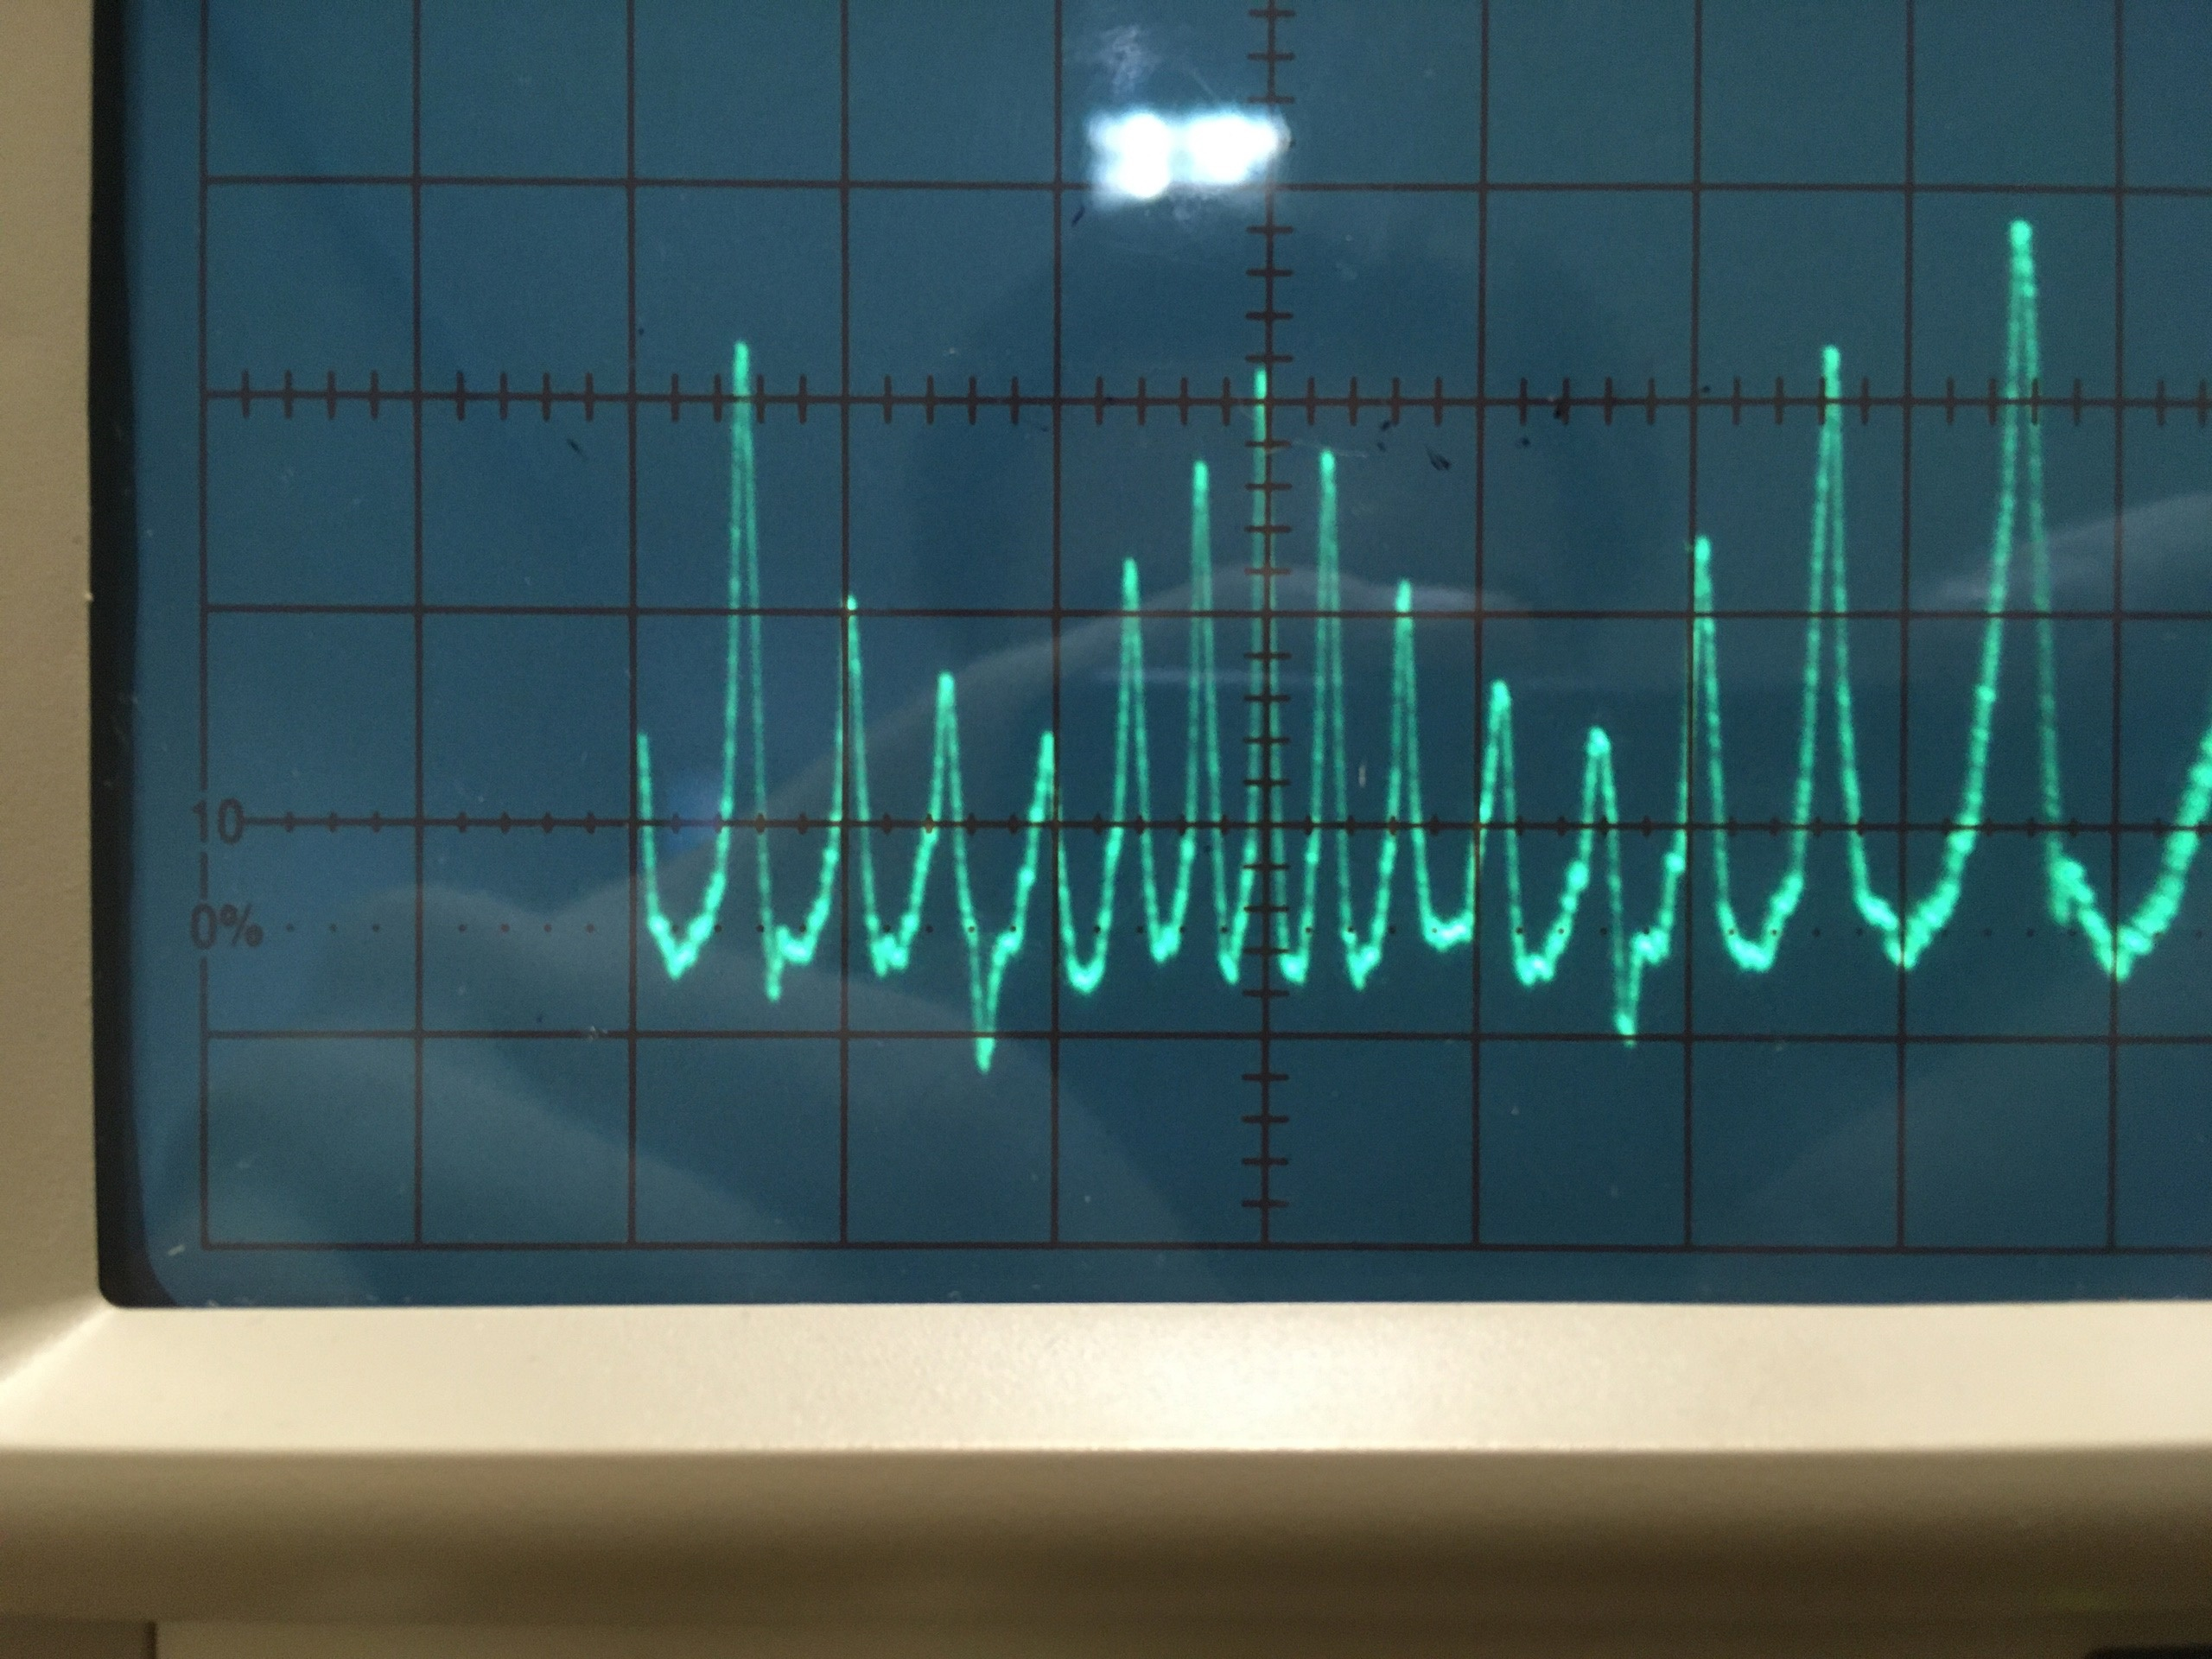
\includegraphics[width=0.5\linewidth]{spectrum_1.jpg}
    \caption{Развертка спектра лазера}\label{fig:spectrum_1}
\end{figure}

На рис.~\ref{fig:spectrum_1} виден удвоенный спектр гауссовского профиля излучения лазера. В одном профиле помещается $N=7$ мод. Полуширина профиля равна:


\begin{equation}
    \Delta\lambda(\text{Ne})=\frac{N}{2} \frac{\lambda^2}{2L} \approx
    10.78 \cdot 10^{-4}\text{ нм}
\end{equation}

Предполагая, что ширина спектральной линии обусловлена эффектом Доплера, можем оценить температуру лазерной трубки.


    $$\frac{\Delta\lambda(\text{Ne})}{\lambda}\approx\frac{v_x}{c}
    \text{;\ \ \ } \frac{m{v_x}^2}{2} \approx \frac{kT}{2}$$
\begin{equation}   
    T \approx \frac{m}{k}\left( \frac{\Delta\lambda(\text{Ne})}{\lambda}\cdot c\right)^2
\end{equation}

Согласно полученным данным получаем температуру трубки $T\approx 634.8$ К.

\item
Дисперсионная область интерферометра, рассчитанная по формуле (\ref{eq:mode_distance_lambda_fabri}): $\Delta\lambda_{\text{си}} \approx 2.22 \cdot 10^{-3} \text{ нм}$. 

Полученное значение очень похоже на удвоенную полуширину профиля: $2\Delta\lambda(\text{Ne}) \approx 2.156 \cdot 10^{-3} \text{ нм}$.

\item
Оценим разрешающую способность интерферометра, измеряя ширину моды на полувысоте.

Расстояние между пиками $2.0$ клетки, что, вычисляя через полуширину профиля, соответствует $$\Delta\lambda = 2\Delta\lambda(\text{Ne})/N = 3.09\cdot10^{-4}\text{ нм}$$
Ширина на полувысоте составляет $0.6$ клетки, что соответствует $$\delta\lambda = \Delta\lambda\cdot\frac{0.6}{2} = 0.92 \cdot 10^{-4}\text{ нм}$$
Разрешающая способность $$R=\frac{\lambda}{\delta\lambda} \approx 6.8\cdot 10^6$$

Разрешающая способность интерферометра Фабри-Перо

\begin{equation}
    R = \frac{2\pi l}{\lambda(1-r)}
\end{equation}

Отсюда можем оценить коэффициент отражения зеркал: $r\approx0.87$

\end{enumerate}

\section{Обсуждение результатов}
По итогу работу, мы выяснили, что газокинетическая температура в разряде составляет $634.8\text{ К} \approx 362 ^\circ\text{C}$, что не соответствует действительности, исходя из ощущений руки вблизи неё. 

Так же стоит заметить, что видимая ширина линии неона (с учетом приближения к полуширине доплеровского контура при расчетах) $2\Delta \lambda\text{(Ne)} = 2.16\cdot10^{-3}\text{ нм}$ практически совпадает с дисперсионной областью сканирующего интерферометра $\Delta \lambda_{\text{си}} = 2.22\cdot10^{-3}\text{ нм}$, что может означать неполное исследование спектра лазера (полоса пропускания интерферометра обрезает спектр лазера).

Разрешающая способность интерферометра $R = 6.8\cdot10^6$ по порядку совпадает со среднестатистическими значениями ($10^6$ и более), но коэффициент отражения зеркал $r \approx 0.87$ маловат для оптического прибора, предназначенного для точных измерений, из чего можно сделать вывод, что и здесь присутствует значительная ошибка.

В целом, на качественном уровне, наблюдения соотносятся с теорией, но установка не приспособлена для количественных измерений.

\end{document}